% L9a lecture companion. Notebook hashes and coverage are recorded in README.md.
% Style files and Cornell seal are copied unchanged from the L7c deck (identical
% to L7a and L6c, which match the approved L6a deck). The linearly separable
% schematic is converted from ../figs/Fig-LinearlySeparable-Schematic.svg to a
% light PDF in assets/ by `make figures`.
%
% Notation follows the lecture: augmented features \hat{x}_i, parameters
% theta = (w_1, ..., w_m, b), labels y in {-1, 1}, and the sign function set
% in typewriter type. Greek vectors (theta) are set plain, as the notebook
% renders them.
\documentclass[aspectratio=169,11pt]{beamer}
\usepackage{vnslides}
\renewcommand{\vnlecturecode}{L9a}
\newcommand{\lecturelink}{https://github.com/varnerlab/CHEME-5800-CourseRepository-Fall-2026/blob/main/weeks/week-09/L9a/CHEME-5800-L9a-Lecture-LinearClassificationAndPerceptron-Fall-2026.ipynb}
\newcommand{\examplelink}{https://github.com/varnerlab/CHEME-5800-CourseRepository-Fall-2026/blob/main/weeks/week-09/L9a/CHEME-5800-L9a-Example-LinearModels-Classification-Perceptron-Fall-2026.ipynb}
\newcommand{\lablink}{https://github.com/varnerlab/CHEME-5800-CourseRepository-Fall-2026/blob/main/weeks/week-09/L9b/CHEME-5800-L9b-Lab-XOR-Fall-2026.ipynb}
\newcommand{\lecturesource}[1]{\note{[Sources]\par
  \href{\lecturelink}{L9a lecture: Linear Models for Classification.}\par
  #1\par[/Sources]}}
\newcommand{\xh}{\hat{\mathbf x}}
\newcommand{\sgn}{\texttt{sign}}
% Strut that gives each displayed fraction in the metrics table room to breathe.
\newcommand{\fracstrut}{\rule[-1.05em]{0pt}{2.75em}}

\title{\texorpdfstring{{\vnheavy L9a}}{L9a}: Linear Models for Classification}
\subtitle{\texorpdfstring{Binary classification, the Perceptron, and the confusion matrix\\[3pt]CHEME 5800 Cornell University}{Binary classification, the Perceptron, and the confusion matrix; CHEME 5800 Cornell University}}
\author{Copyright Jeffrey Varner 2026. All Rights Reserved}

\begin{document}
\special{pdf:minorversion 7}
\vntitlepage

\begin{frame}{Objectives for Today}
  How can a linear model assign each example to one of two classes, and how
  do we judge the labels it assigns?

  \vspace{0.4em}
  {\large\textbf{\ink{Today's concepts}}}
  \vspace{0.2em}
  \begin{itemize}\setlength{\itemsep}{0.4em}
    \item \hilite{Adapt a linear model for binary classification}: pass its
      output through the sign function to get a class label, and see how the
      parameters define a boundary between the two classes.
    \item \hilite{Train a linear classifier with the Perceptron algorithm}:
      update the parameters only on mistakes, show why each update helps, and
      see when the algorithm is guaranteed to separate the classes.
    \item \hilite{Evaluate a classifier with a confusion matrix}: compute
      accuracy, precision, recall, and specificity, and see why accuracy alone
      can mislead when one class is rare.
  \end{itemize}
  \slidenote{Lecture:}{\href{\lecturelink}{Linear Models for Classification}}
  \lecturesource{Introduction and three Learning Objectives.}
\end{frame}

\begin{frame}{Lecture and Example}
  \textbf{\ink{Lecture:}}
  \href{\lecturelink}{Linear Models for Classification}

  In this lecture, we turn a linear model into a binary classifier, train it
  with the Perceptron algorithm, and evaluate its predictions with a
  confusion matrix.

  \vspace{1.1em}
  \textbf{\ink{Example:}}
  \href{\examplelink}{Build a Perceptron Classifier}

  In this example, we train the Perceptron to tell genuine banknotes from
  forged ones, classify banknotes it has not seen, and use a confusion matrix
  to see which kinds of errors it makes.
  \lecturesource{Introduction and Examples.}
\end{frame}

\begin{frame}{Binary Classification Problem}
  In a \hilite{binary classification} problem, each example belongs to one of
  two classes, and we want to predict the class from the example's features.
  A linear model computes a continuous output, a \hilite{score}, from the
  features. An \hilite{activation function} $\sigma$ transforms the score
  either directly into a class label or into the probability of each class.

  \vspace{0.6em}
  \begin{itemize}\setlength{\itemsep}{0.7em}
    \item \hilite{The Perceptron} (Rosenblatt, 1957) learns a linear decision
      boundary and maps the score directly to a class label in $\{-1,+1\}$
      with $\sigma(z)=\sgn(z)$.
    \item \hilite{Logistic regression} uses the logistic function, an S-shaped
      curve with values between $0$ and $1$, to turn the score into the
      probability that an example belongs to a class.
  \end{itemize}

  \vspace{0.6em}
  Today, we focus on the Perceptron.
  \lecturesource{Binary Classification Problem: opening paragraph and the two strategies.}
\end{frame}

\begin{frame}{Linearly Separable Data}
  Each point is an example with two features, colored by its class.

  \vspace{0.3em}
  \centering
  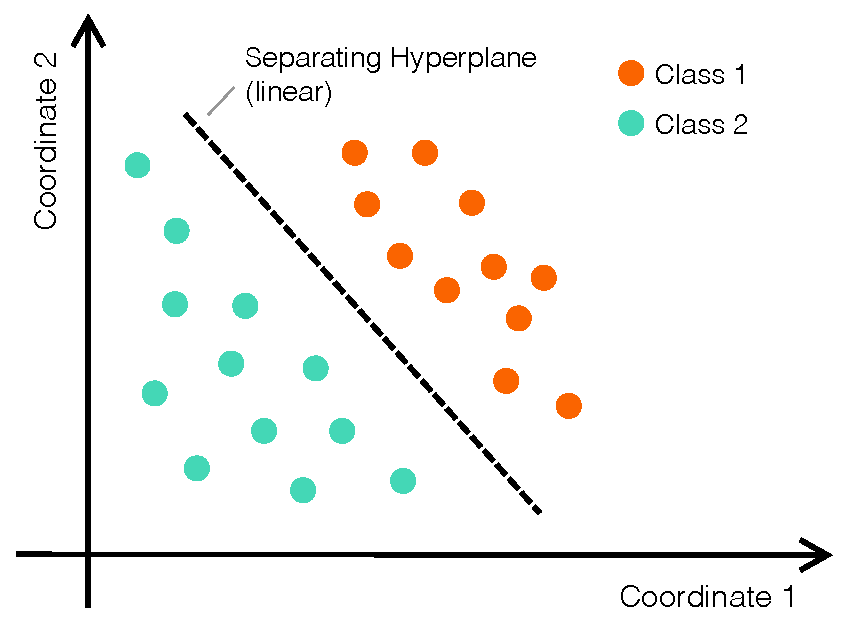
\includegraphics[width=\textwidth,height=0.52\paperheight,keepaspectratio]{assets/Fig-LinearlySeparable-Schematic.pdf}

  \vspace{0.3em}
  \raggedright
  These data are \hilite{linearly separable}: a straight boundary puts every
  class 1 example on one side and every class 2 example on the other.
  \lecturesource{Binary Classification Problem: figure and caption.
    Figure: ../figs/Fig-LinearlySeparable-Schematic.svg, converted to a light PDF with rsvg-convert.}
\end{frame}

\begin{frame}{The Perceptron Classifier}
  Suppose a dataset $\mathcal D=\{(\mathbf x_i,y_i)\mid i=1,\ldots,n\}$ has $n$
  labeled examples, with features $\mathbf x_i\in\mathbb R^m$ and a class label
  $y_i\in\{-1,1\}$. The Perceptron estimates the label by passing the linear
  score through the sign function:
  \[
    \hat y_i=\sgn\bigl(\xh_i^\top\theta\bigr),
    \qquad
    \sgn(z)=
    \begin{cases}
      1 & \text{if } z\ge0,\\
      -1 & \text{if } z<0,
    \end{cases}
  \]
  where the augmented features $\xh_i^\top=(x_{i1},\ldots,x_{im},1)$ add a $1$
  for the bias term, so $p=m+1$, and $\theta=(w_1,\ldots,w_m,b)\in\mathbb R^p$
  holds the weight $w_j$ of each feature and the bias $b$.
  \lecturesource{Perceptron: dataset, estimated label, augmented features, and the sign function.}
\end{frame}

\begin{frame}{Decision Boundary and Mistakes}
  The \hilite{decision boundary} is the set of feature vectors where the score
  is zero:
  \[
    \bigl\{\mathbf x\in\mathbb R^m\mid\xh^\top\theta=w_1x_1+\cdots+w_mx_m+b=0\bigr\}.
  \]
  The score is positive on one side and negative on the other. When at least
  one weight is nonzero, the boundary is a \hilite{hyperplane}: a line when
  $m=2$ and a plane when $m=3$. The weights set its orientation, and the bias
  shifts it away from the origin.

  \vspace{0.6em}
  The product $y_i\,\xh_i^\top\theta$ is positive when example $i$ is on the
  correct side, and example $i$ is a \hilite{mistake} when
  $y_i\,\xh_i^\top\theta\le0$: on the wrong side or on the boundary. The dataset is \hilite{linearly separable} if some $\theta$ makes
  this product positive for every example.
  \lecturesource{Perceptron: Decision boundary paragraph and the mistake and linear-separability definitions.}
\end{frame}

\begin{frame}{Online Perceptron Training}
  \textbf{Initialize}: Given $\mathcal D$, a pass limit $T\ge1$, and a mistake
  threshold $M$ (e.g., $M=0$), set $\theta=(w_1,\ldots,w_m,b)$ to zero or small
  random values and the loop counter $t\gets0$.

  \vspace{0.4em}
  While $\texttt{true}$ \textbf{do}:
  \begin{enumerate}\setlength{\itemsep}{0.25em}
    \item Initialize the number of mistakes $\texttt{mistakes}\gets0$.
    \item For each training example $(\mathbf x,y)\in\mathcal D$, with augmented
      features $\xh$, \textbf{do}:
      \begin{itemize}\setlength{\itemsep}{0.1em}
        \item If $y\,\xh^\top\theta\le0$, \textbf{then} the example is a
          mistake. Update $\theta\gets\theta+y\,\xh$ and increment
          $\texttt{mistakes}\gets\texttt{mistakes}+1$.
      \end{itemize}
    \item After processing all examples, increment $t\gets t+1$.
    \item If $\texttt{mistakes}\le M$ \textbf{or} $t\ge T$, \textbf{then} return
      $\theta$. Otherwise, repeat from step 1.
  \end{enumerate}

  \vspace{0.3em}
  The Perceptron is an \hilite{online} algorithm: it looks at one example at a
  time and updates $\theta$ right after each mistake.
  \lecturesource{Classical: Online Perceptron Training: pseudocode. Preserve the Initialize/While/numbered-step format.}
\end{frame}

\begin{frame}{Why Does the Update Help?}
  Suppose the example $(\mathbf x,y)$ is a mistake, and let
  $\theta'=\theta+y\,\xh$ be the updated parameters. Because $y^2=1$:
  \[
    y\,\xh^\top\theta'
    =y\,\xh^\top\theta+y^2\,\xh^\top\xh
    =y\,\xh^\top\theta+\|\xh\|_2^2.
  \]

  \vspace{0.4em}
  \begin{itemize}\setlength{\itemsep}{0.7em}
    \item \hilite{The product grows} by $\|\xh\|_2^2$, the squared length of
      $\xh$, which is at least $1$ because the last entry of $\xh$ is $1$.
      The update moves this example's score toward the correct sign.
    \item \hilite{One update may not be enough}: the product may still be
      negative, and the update also changes the scores of the other examples.
      So we pass through the data repeatedly.
  \end{itemize}
  \lecturesource{Classical: Online Perceptron Training: Why does this update help?}
\end{frame}

\begin{frame}{Perceptron Convergence Theorem}
  \textbf{Novikoff (1962).} Suppose that:
  \begin{itemize}\setlength{\itemsep}{0.4em}
    \item \hilite{Margin}: some $\theta^\star$ with $\|\theta^\star\|_2=1$ gives
      $y_i\,\xh_i^\top\theta^\star\ge\gamma>0$ for every example.
    \item \hilite{Radius}: $R=\max_i\|\xh_i\|_2$ is the length of the longest
      augmented feature vector.
  \end{itemize}
  Then, starting from $\theta=\mathbf 0$, the number of updates $k$ satisfies:
  \[
    \boxed{k\le\left(\frac{R}{\gamma}\right)^{2}}
  \]

  \vspace{0.3em}
  A larger margin $\gamma$ lowers the bound. On separable data, with $M=0$ and
  a large enough $T$, the Perceptron stops after finitely many updates.
  \lecturesource{Classical: Online Perceptron Training: Convergence paragraph and the Perceptron convergence theorem callout.}
\end{frame}

\begin{frame}{When Does the Perceptron Stop?}
  \begin{itemize}\setlength{\itemsep}{0.8em}
    \item \hilite{Separable data}: a pass with zero mistakes leaves $\theta$
      unchanged, so the returned $\theta$ classifies every training example
      correctly.
    \item \hilite{Data that are not separable}: every pass makes at least one
      mistake, so with $M=0$ the loop runs until it reaches the limit of $T$
      passes.
    \item \hilite{In practice}: we rarely know in advance whether the data are
      separable. That is why the algorithm always has a pass limit $T$, and
      why we may stop after a pass with at most $M>0$ mistakes.
  \end{itemize}

  \vspace{0.8em}
  Another way to train a linear classifier is to write a loss function that
  measures the classification error and minimize it with numerical optimization.
  \lecturesource{Classical: Online Perceptron Training: paragraph after the convergence theorem, and Modern: Nonlinear Optimization.}
\end{frame}

\begin{frame}{Confusion Matrix for Binary Classification}
  A \hilite{confusion matrix} compares predicted labels with actual labels.
  We call the class we want to detect \hilite{positive} ($y=1$) and the other
  class \hilite{negative} ($y=-1$):

  \vspace{0.6em}
  \centering
  \begin{tabular}{lll}
    \toprule
    & \textbf{Predicted positive} & \textbf{Predicted negative}\\
    \midrule
    \textbf{Actual positive} & True positive (TP) & False negative (FN)\\
    \textbf{Actual negative} & False positive (FP) & True negative (TN)\\
    \bottomrule
  \end{tabular}

  \vspace{0.8em}
  \raggedright
  The diagonal entries count the correct predictions, and the off-diagonal
  entries count the two kinds of mistakes.

  \vspace{0.5em}
  In medical diagnosis, a \hilite{false positive} tells a healthy patient they
  have the disease, while a \hilite{false negative} misses a patient who has it.
  The two mistakes can have very different costs, so we count them separately.
  \lecturesource{Confusion Matrix for Binary Classification: structure callout and the medical-diagnosis paragraph.}
\end{frame}

\begin{frame}{Performance Metrics}
  The confusion matrix gives the counts for four performance metrics:

  \vspace{0.5em}
  \centering
  {\small\setlength{\tabcolsep}{4.5pt}%
  \begin{tabular}{lcl}
    \toprule
    \textbf{Metric} & \textbf{Formula} & \textbf{What it measures}\\
    \midrule
    \hilite{Accuracy} & \fracstrut$\dfrac{TP+TN}{TP+TN+FP+FN}$ & Fraction of all predictions that are correct\\
    \hilite{Precision} & \fracstrut$\dfrac{TP}{TP+FP}$ & Fraction of positive predictions that are correct\\
    \hilite{Recall (sensitivity)} & \fracstrut$\dfrac{TP}{TP+FN}$ & Fraction of actual positives the classifier finds\\
    \hilite{Specificity} & \fracstrut$\dfrac{TN}{TN+FP}$ & Fraction of actual negatives labeled negative\\
    \bottomrule
  \end{tabular}}

  \vspace{0.7em}
  \raggedright
  Accuracy can mislead when one class is rare: if 3\% of examples are positive,
  always predicting negative is 97\% accurate, with zero recall.
  \lecturesource{Confusion Matrix for Binary Classification: Performance Metrics and the Key insight callout.}
\end{frame}

\begin{frame}{Example: Build a Perceptron Classifier}
  In this example, we classify 1{,}372 genuine and forged banknotes from four
  numerical features computed from a camera image of each note.

  \vspace{0.4em}
  \begin{enumerate}\setlength{\itemsep}{0.55em}
    \item Train the Perceptron on the training banknotes, which are not linearly
      separable, and keep the best parameters with the \hilite{pocket algorithm}.
    \item Classify the testing banknotes, which the Perceptron never saw, and
      compare the testing and training mistake rates.
    \item Compute the confusion matrix for the testing banknotes, with forged
      banknotes as the positive class, and the four performance metrics.
  \end{enumerate}

  \vspace{0.4em}
  A false negative accepts a forgery as genuine; a false positive flags a
  genuine banknote as forged.
  \slidenote{Example:}{\href{\examplelink}{Build a Perceptron classifier}}
  \lecturesource{Confusion Matrix for Binary Classification: example callout.
    Companion example: Tasks 1--3, the pocket algorithm subsection, and the Error analysis callout.}
\end{frame}

\begin{frame}{Lab: The Perceptron on XOR}
  In the \href{\lablink}{lab}, we train the Perceptron on datasets that are and are
  not linearly separable, including the \hilite{XOR} (exclusive or) pattern:

  \vspace{0.6em}
  \begin{itemize}\setlength{\itemsep}{0.5em}
    \item the feature plane is cut into four wedges, and diagonally opposite
      wedges share a class,
    \item no straight line separates the classes, so every pass makes a mistake,
    \item we compare the learned boundaries and the test performance, with and
      without the \hilite{pocket algorithm}.
  \end{itemize}

  \vspace{0.6em}
  Minsky and Papert's 1969 proof that the Perceptron cannot learn XOR became
  a central point of their critique.
  \slidenote{Lab:}{\href{\lablink}{The Perceptron on non-linearly separable data}}
  \lecturesource{Lab section. Lab notebook: introduction, Backstory, and Learning Objectives.}
\end{frame}

\begin{frame}{Summary}
  We adapted linear models for binary classification, trained a linear
  classifier with the Perceptron, and evaluated it with a confusion matrix.

  \vspace{0.6em}
  {\large\textbf{\ink{Key takeaways}}}
  \vspace{0.3em}
  \begin{itemize}\setlength{\itemsep}{0.65em}
    \item \textbf{\ink{Linear models for classification.}} We passed the linear
      score through the sign function to get a class label; the parameters
      define the decision boundary between the two classes.
    \item \textbf{\ink{Perceptron learning and convergence.}} We showed that each
      update moves a mistake's score toward the correct sign, so on separable
      data the Perceptron stops after finitely many updates.
    \item \textbf{\ink{Performance evaluation.}} We used the confusion matrix
      counts to compute four metrics and saw that accuracy alone can hide a
      classifier that misses a rare class.
  \end{itemize}

  \vspace{0.8em}
  The example and lab apply these ideas to banknotes and to the XOR pattern.
  \lecturesource{Summary: three key takeaways and concluding sentence.}
\end{frame}

\end{document}
